% fig_I0_earthing.tex
% TR-25: Bar chart — I0_diff and I2_diff vs fault type × earthing
% Shows that I0 is significant for earthed SLG, I2 is not (pure IBR)
% Three groups: E1 Solid, E2 R-earth, E3 Unearthed
% Two bars per group: I0_diff (blue) and I2_diff (orange)
% Horizontal line: I0_thr=0.04, I2_thr=0.06
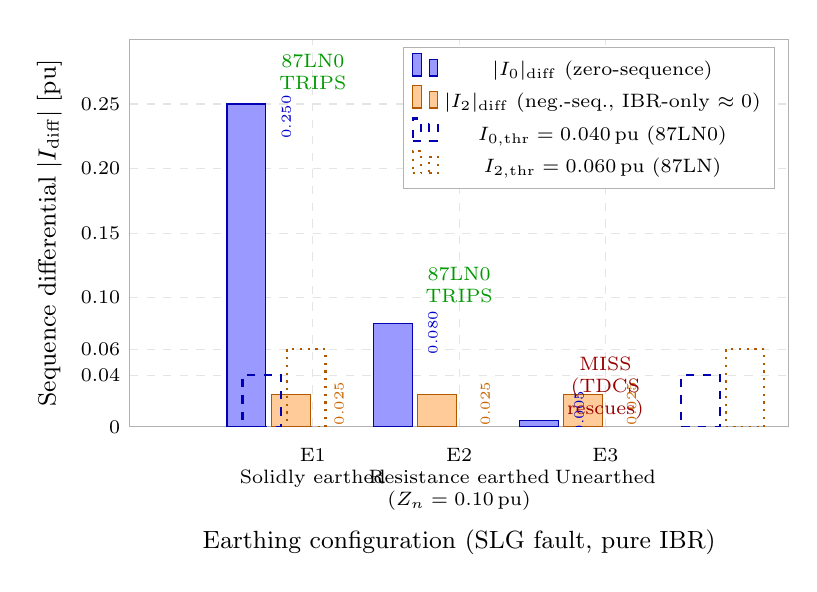
\begin{tikzpicture}
\begin{axis}[
  name       = i0ax,
  ybar,
  bar width  = 14pt,
  width      = 0.82\textwidth,
  height     = 6.5cm,
  ylabel     = {Sequence differential $|I_{\rm diff}|$ [pu]},
  ylabel style={font=\small},
  xlabel     = {Earthing configuration (SLG fault, pure IBR)},
  xlabel style={font=\small},
  ymin=0, ymax=0.30,
  ytick      = {0, 0.04, 0.06, 0.10, 0.15, 0.20, 0.25},
  yticklabels= {0, 0.04, 0.06, 0.10, 0.15, 0.20, 0.25},
  yticklabel style={font=\scriptsize},
  xtick      = {1, 2, 3},
  xticklabels= {E1\\Solidly earthed,
                E2\\Resistance earthed\\($Z_n=0.10$\,pu),
                E3\\Unearthed},
  xticklabel style={font=\scriptsize, align=center},
  enlarge x limits=0.25,
  legend style={at={(0.98,0.98)}, anchor=north east,
                font=\scriptsize, draw=gray!60},
  grid       = major,
  grid style = {gray!20, dashed},
  tick style = {draw=none},
  axis line style={gray!60},
]

% I0_diff bars (blue): 0.250, 0.080, 0.005
\addplot[fill=blue!40, draw=blue!70!black]
  coordinates { (1, 0.250) (2, 0.080) (3, 0.005) };
\addlegendentry{$|I_0|_{\rm diff}$ (zero-sequence)}

% I2_diff bars (orange, near zero for pure IBR): 0.025, 0.025, 0.025
\addplot[fill=orange!40, draw=orange!70!black]
  coordinates { (1, 0.025) (2, 0.025) (3, 0.025) };
\addlegendentry{$|I_2|_{\rm diff}$ (neg.-seq., IBR-only $\approx 0$)}

% I0 threshold = 0.04 pu
\addplot[blue!70!black, thick, dashed, mark=none, domain=0.5:3.5, samples=2]
  ({x}, {0.040});
\addlegendentry{$I_{0,\rm thr}=0.040$\,pu (87LN0)}

% I2 threshold = 0.06 pu
\addplot[orange!70!black, thick, dotted, mark=none, domain=0.5:3.5, samples=2]
  ({x}, {0.060});
\addlegendentry{$I_{2,\rm thr}=0.060$\,pu (87LN)}

% Value labels
\node[font=\tiny, blue!80!black, rotate=90] at (axis cs:0.82, 0.240) {0.250};
\node[font=\tiny, blue!80!black, rotate=90] at (axis cs:1.82, 0.073) {0.080};
\node[font=\tiny, blue!80!black, rotate=90] at (axis cs:2.82, 0.011) {0.005};
\node[font=\tiny, orange!80!black, rotate=90] at (axis cs:1.18, 0.018) {0.025};
\node[font=\tiny, orange!80!black, rotate=90] at (axis cs:2.18, 0.018) {0.025};
\node[font=\tiny, orange!80!black, rotate=90] at (axis cs:3.18, 0.018) {0.025};

% Trip/no-trip indicators
\node[font=\scriptsize, green!60!black, align=center] at (axis cs:1.0, 0.275)
  {87LN0\\TRIPS};
\node[font=\scriptsize, green!60!black, align=center] at (axis cs:2.0, 0.110)
  {87LN0\\TRIPS};
\node[font=\scriptsize, red!60!black, align=center] at (axis cs:3.0, 0.030)
  {MISS\\(TDCS\\rescues)};

\end{axis}
\end{tikzpicture}
